\section{Logical approaches to movement}%
\label{sec:movement-and-quantifier-raising}
In this section, we will discuss logical approaches to
quantification. We will start out by describing the problem of
quantification. Then we will discuss the choice between semantic and
syntactic approaches. Next, we will discuss the existing semantic
approaches to quantifier raising, and why they are inadequate. We will
then discuss various syntactic approaches to quantifier raising, and
finish by making our own contributions.

\subsection{Quantification in natural language}
Quantification is the problem of analysing scope-taking expressions in
natural language. For instance, the canonical interpretation for a
sentence such as ``Everyone laughs'' is:
\[
  \forall{x}.\PERSON(x)\supset\LAUGH(x)
\]
The problem here, is that the quantifier ``everyone'' is ostensibly an
NP. However, in the given semantics, it is taking scope over
``laughs''. A more obvious version of this problem can be seen in
``John [saw everyone]'', where the quantifier is more deeply nested in
the parse tree:
\[
  \forall{y}.\PERSON(y)\supset\PAST(\SEE(\JOHN,y))
\]
The problem becomes even more interesting when you consider sentences
with multiple quantifiers. Here we observe a phenomenon known as
\emph{scope ambiguity}. The canonical example is the phrase ``Everyone
loves someone'', which has the following interpretations:
\begin{alignat*}{3}
  &\forall x.\PERSON(x) \,&\supset \,&\exists y.\PERSON(y) \,&\wedge  \,&\LIKE(x,y)\\
  &\exists y.\PERSON(y) \,&\wedge  \,&\forall x.\PERSON(x) \,&\supset \,&\LIKE(x,y)
\end{alignat*}

There are several easy ways to obtain these semantics within the
type-logical grammar that we have established in
\autoref{sec:introduction} and \autoref{sec:lexical-ambiguity}.
One approach, due to \citet{montague1973}, is to assign NP the
semantic type $(\e\t)\t$. This way, we can define the lexicon as
follows:
\begin{alignat*}{3}
  &\text{john}     &&= \lambda k. k\;\JOHN                          \\
  &\text{everyone} &&= \lambda k. \forall x. \PERSON(x)\supset k\;x \\
  &\text{laughs}   &&= \lambda x. x\;\LAUGH
\end{alignat*}
We can even build in scope ambiguity by assigning ``loves'' an
  ambiguous type---e.g., using the extension from
  \autoref{sec:lexical-ambiguity}, we assign it the type $\TV\&\TV$,
  and define it as:
\[
  \text{loves} = \lambda k_2. \lambda k_1.
  (k_1\;(\lambda x.k_2\;(\lambda y.\LOVE(x,y))), k_2\;(\lambda y.k_1\;(\lambda x.\LOVE(x,y)))
\]
However, somehow it feels wrong to manually build scope ambiguity into
every verb: it is a universal property of language, so it should not
be encoded in the lexicon, but in our type-logical grammar.

It is also quite odd that we give ``john''---which by all measures is
not a quantifier---the freedom to act as a quantifier. And because we
do not distinguish between quantificational and non-quantificational
NPs, we are left with a large amount of scope ambiguity---spurious
ambiguity. For instance, the sentences ``Mary likes John'' will be
considered ambiguous, with both interpretations equal to $\LIKE(\MARY,
\JOHN)$. \citet{hendriks1993} a solution to this problem, developing a
framework in which terms are lifted into quantificational terms only
when this is needed.

\todo{How does \citet{hendriks1993} deal with scope ambiguity?}

\vspace*{1\baselineskip}

Another approach---popular in associative Lambek calculi---is to use
higher-order syntactic types. For instance, we can assign ``everyone''
the syntactic type $\S\impl\IV$. This also gives us the semantic type
$(\e\t)\t$, and therefore we are able to assign it the same term as
before. This works perfectly for sentences with subject-quantifiers,
and it \emph{does} distinguish between quantificational and
non-quantificational NPs, but it has one downside: it does not work
for sentences with object-quantifiers.
In the \emph{associative} Lambek calculus, we can use the similar
looking type $(\S\impl\NP)\impr\S$---a similarity which extended the
popularity of the associative Lambek calculus way past its due
date. Meanwhile, in NL, we have to devise a type which actually
reflects the sentence structure, such as $\TV\impr\IV$. Using
this type, we can assign ``everyone'' a second interpretation:
\[
  \text{everyone} = \lambda k.\lambda x.\forall y.\PERSON(y)\supset(k\;y\;x)
\]
The need for multiple definitions for `everyone' aside, there are more
problems with this approach: with our current definitions for
``everyone''---and similar definitions for ``someone''---we can only
derive the first of the two expected interpretations for ``Everyone
likes someone''.
Now, we could imagine giving a third definition for ``everyone'' and
``someone'', with the type $(\TV\impr((\S\impl\IV)\impr\IV))$, which
would allow us to define object quantifiers taking scope over subject
quantifiers. However, there are many other cases---think of
ditransitive verbs, or verb phrases modified by some number of
adverbs. Clearly, this is not an elegant solution, as we are basically
hard-coding the structures that quantifiers can take scope over in
their types.

\vspace*{1\baselineskip}

One interesting aspect of the two approaches we have discussed so far
is that they very clearly divide in a semantic and a syntactic
approach. The first approach was implemented in the translation to
semantic types, and in the lexicon. The second approach was
implemented entirely within the syntactic calculus. With any
linguistic phenomenon this is an important question: do we consider it
to be syntactic or semantic in nature? With quantification, the
community seems divided. In this thesis, we will approach the problem
of quantification as a syntactic phenomenon. Therefore, in the
next section we will discuss some of the approaches to quantification
as a semantic problem, and their limitations. Following this, we will
discuss various approaches to quantification as a syntactic problem,
discuss their weaknesses, and try to amend these.


\subsection{Semantic approaches to scope taking}
\label{sec:continuations-and-scope-taking}



\subsubsection{Continuation-passing style translation}
\citet{barker2002,barker2004} advocates the use of continuations in
natural language semantics. He does this with several case studies,
one of which is quantification. The gist of his story is as follows:

As mentioned before, in the sentence ``John [saw everyone]'', the
deeply nested quantifier ``everyone'' must take scope over the
remainder of the sentence. Instead of translating NP to the higher-order
type $(\e\t)\t$, \citeauthor{barker2002} proposes to lift \emph{every
  type}, consistently, using a technique from computer science known
as continuation-passing style (CPS) translation. After translating the
syntactic terms, he applies a CPS-translation, lifting expressions of
type $A$ into the type $(A\ra R)\ra R$ for some answer type $R$. He
assumes that the function-argument structure that is the result of
the translation to syntactic terms is constructed using only variables
and function application,\footnote{%
  This is equivalent to restricting the syntactic calculus to the
  applicative, i.e.\ Ajdukiewicz-Bar-Hillel fragment
  \citep[see][ch.\ 1.1-1.5, AB-grammars]{moot2012}.
}
and defines the translation as follows:\footnote{%
  It should be noted that \citeauthor{barker2004}'s initial solution
  uses some directional information to ensure that scope-takers are
  always processed in a left-to-right order, instead of always
  processing the argument first, as it is presented here.
  This distinction, however, becomes irrelevant once he introduces the
  ambiguous translation, and therefore I have chosen not to include it.
}
\begin{alignat*}{3}
  &\overline{x}    &&= x\\
  &\overline{M\;N} &&= \lambda k. \overline{N}\;(\lambda n.\overline{M}\;(\lambda m.k\;(m\;n)))
\end{alignat*}
This translation is applied to the function-argument structure
\emph{before} lexical definitions are inserted.
In addition, the lexical items have to be lifted manually for this to
work---although the lifting is a much simpler process:
\begin{alignat*}{3}
  &\text{john}     &&= \lambda k. k\;\JOHN                          \\
  &\text{everyone} &&= \lambda k. \forall x. \PERSON(x)\supset k\;x \\
  &\text{laughs}   &&= \lambda k. k\;\LAUGH                         \\
  &\text{loves}    &&= \lambda k. k\;\LOVE
\end{alignat*}
However, this analysis of quantification has several issues. The first
of these is already mentioned by \citet{barker2004}: scope ambiguity.
The solution provided by \citet{barker2002,barker2004} will only
derive the surface-scope interpretation of ``Everyone loves
someone''. Barker solves this problem by making the CPS-translation
ambiguous, adding another possible translation for function
application:
\begin{alignat*}{3}
  &\overline{x}    &&= x\\
  &\overline{M\;N} &&= \lambda k. \overline{N}\;(\lambda n.\overline{M}\;(\lambda m.k\;(m\;n)))\\
  &\overline{M\;N} &&= \lambda k. \overline{M}\;(\lambda m.\overline{N}\;(\lambda n.k\;(m\;n)))
\end{alignat*}
\note{Barker's CPS-translation \emph{is} recursive. However, he has a
  strange way of presenting it. Instead of performing the translation
  on the function-argument structure, he defines a new type of
  application, and hides the recursion in there.}
This does solve the problem at hand, and derives both the
surface-scope and the inverse-scope interpretations. However, this
solution results in a huge amount of spurious ambiguity.
A sentence with $n$ words has $n-1$ function applications, and will
therefore have $2^{(n-1)}$ interpretations. But this ambiguity is only
relevant for scope-takers.
In the motivating example, ``loves'' is not a scope
taker. Nevertheless, it is treated as one, which means there are two
possible translations for ``loves someone'', resulting in four
interpretations for the sentence where we only want two. This
ambiguity grows exponentially with the length of the sentence.

% Secondly, using an ambiguous translation clearly makes our
% CPS-translation incompatible with our monadic translation, unless we
% are willing to ambiguously translate all our effects. But doing so
% is risky, as a right-to-left interpretation may not be desirable for
% effects other than quantification. For instance, a right-to-left
% interpretation of the state monad for anaphora resolution will allow
% sentences such as ``He$_i$ gave a book to John$_i$.''



\subsubsection{Focused, polarised semantics}
Instead of performing a separate CPS translation on the semantic
terms, \citet{bastenhof2012}, \citet{moortgat2012}---based on work by
\citet{girard1991} and \citet{curien2000}---integrate the
CPS-semantics into the syntactic calculus. The result of this work is
the focused Lambek-Grishin (LG) calculus, a bilinear variant of NL,
with semantics inspired on \citepos{parigot1992}
$\lambda\mu$-calculus. Focused NL, as presented in this thesis, is a
fragment of focused LG. Below we will present the CPS-semantics for
the the product-free NL fragment of focused LG. First of all, the
translation on types. Let $A^R= A\ra R$:
\[
  \begin{aligned}
    &\llbracket\alpha\rrbracket^+ &&=
    \begin{cases}
      \phantom{((}\tr[\alpha] &\mbox{if } \text{Pol}(\alpha)\equiv{+}\\
      ((\tr[\alpha])^R)^R &\mbox{if } \text{Pol}(\alpha)\equiv{-}\\
    \end{cases}
    \quad
    &&\llbracket\alpha\rrbracket^- &&=
    (\tr[\alpha])^R
    \\
    &\llbracket A\impr B\rrbracket^+  &&=
    (\llbracket A\rrbracket^+\times\llbracket B\rrbracket^-)^R
    \quad
    &&\llbracket A\impr B\rrbracket^- &&=
    \llbracket A\rrbracket^+\times\llbracket B\rrbracket^-
    \\
    &\llbracket B\impl A\rrbracket^+  &&=
    (\llbracket B\rrbracket^-\times\llbracket A\rrbracket^+)^R
    \quad
    &&\llbracket B\impl A\rrbracket^- &&=
    \llbracket B\rrbracket^-\times\llbracket A\rrbracket^+
  \end{aligned}
\]
We extend this translation to structures by translating \emph{all}
structural connectives as product types. We translate atomic
\emph{positive} structures using $\llbracket\cdot\rrbracket^+$, and
atomic \emph{negative} structures using
$\llbracket\cdot\rrbracket^-$. We extend it to sequents as follows:
\[
  \begin{aligned}
    &\llbracket\;\,{Γ}\,\,\fCenter\:\,{Δ}\:\,\rrbracket &&=
    \llbracket{Γ\:}\rrbracket\fCenter\llbracket{Δ}\rrbracket^R
    \\
    &\llbracket\focus{A}\fCenter\,\,{Δ}\:\,\rrbracket &&=
    \llbracket{Δ}\rrbracket\fCenter\llbracket{A}\rrbracket^-
    \\
    &\llbracket\;\,{Γ}\,\,\fCenter\focus{B}\;\!\rrbracket &&=
    \llbracket{Γ\:}\rrbracket\fCenter\llbracket{B}\rrbracket^+
  \end{aligned}
\]
As the translations on sequents and types makes the CPS-semantics for
focused NL a somewhat obtuse, we will present them a little more
explicitly that usual. Below, we will give the full derivations for
the translations of the focusing and unfocusing rules, and some
examples for the remaining rules.

Note that for \emph{positive} $A$, $\llbracket{A}\rrbracket^- \equiv
(\llbracket{A}\rrbracket^+)^R$, and for \emph{negative} $A$,
$\llbracket{A}\rrbracket^+ \equiv (\llbracket{A}\rrbracket^-)^R$.
Using these facts, we can give the focusing and defocusing rules a
valid term labelling. In fact, the left focusing and unfocusing rules
are the \emph{only} rules whose translation involves abstraction and
application:
\begin{center}
  \renewcommand{\arraystretch}{1}
  \begin{tabular}{c c}
    \multicolumn{1}{l}{Foc$^R$:} & \multicolumn{1}{l}{Foc$^L$:}
    \\
    \begin{pfbox}
      \AXC{$\llbracket x:Γ\fCenter \focus{M:A} \rrbracket$}
      \UIC{$x:\llbracket Γ\rrbracket\fCenter M:\llbracket A\rrbracket^+$}
      \RightLabel{$\equiv$}
      \UIC{$x:\llbracket Γ\rrbracket\fCenter M:\llbracket A\rrbracket^{-R}$}
      \UIC{$\llbracket x:Γ\fCenter M:\struct{A} \rrbracket$}
    \end{pfbox}
    &
    \begin{pfbox}
      \AXC{}\RightLabel{Ax}
      \UIC{$k:\llbracket A\rrbracket^{-R}\fCenter k:\llbracket A\rrbracket^{-R}$}
      \AXC{$\llbracket\focus{M:A}\fCenter x:Δ\rrbracket$}
      \UIC{$\llbracket x:Δ\rrbracket\fCenter\llbracket M:A\rrbracket^-$}
      \RightLabel{$\ra$E}
      \BIC{$k:\llbracket A\rrbracket^{-R}\prod x:\llbracket Δ\rrbracket\fCenter (k\;M):R$}
      \RightLabel{$\ra$I}
      \UIC{$k:\llbracket A\rrbracket^{-R}\fCenter (\lambda x.k\;M):\llbracket Δ\rrbracket^R$}
      \RightLabel{$\equiv$}
      \UIC{$k:\llbracket A\rrbracket^+\fCenter (\lambda x.k\;M):\llbracket Δ\rrbracket^R$}
      \UIC{$\llbracket k:\struct{A}\fCenter (\lambda x.k\;M):Δ\rrbracket$}
    \end{pfbox}
    \\
    \multicolumn{1}{l}{Unf$^R$:} & \multicolumn{1}{l}{Unf$^L$:}
    \\
    \begin{pfbox}
      \AXC{$\llbracket x:Γ\fCenter\struct{M:A}\rrbracket$}
      \UIC{$\llbracket x:Γ\rrbracket\fCenter M:\llbracket A\rrbracket^{-R}$}
      \RightLabel{$\equiv$}
      \UIC{$\llbracket x:Γ\rrbracket\fCenter M:\llbracket A\rrbracket^+$}
      \UIC{$\llbracket x:Γ\fCenter\focus{M:A}\rrbracket$}
    \end{pfbox}
    &
    \begin{pfbox}
      \AXC{$\llbracket x:\struct{A}\fCenter M:Δ\rrbracket$}
      \UIC{$x:\llbracket A\rrbracket^+\fCenter M:\llbracket Δ\rrbracket^R$}
      \AXC{}\RightLabel{Ax}\UIC{$y:\llbracket Δ\rrbracket\fCenter y:\llbracket Δ\rrbracket$}
      \RightLabel{$\ra$E}
      \BIC{$x:\llbracket A\rrbracket^+\prod y:\llbracket Δ\rrbracket\fCenter (M\;y):R$}
      \RightLabel{Comm.}
      \UIC{$y:\llbracket Δ\rrbracket\prod x:\llbracket A\rrbracket^+\fCenter (M\;y):R$}
      \RightLabel{$\ra$I}
      \UIC{$y:\llbracket Δ\rrbracket\fCenter\llbracket (\lambda x.M\;y):A\rrbracket^{+R}$}
      \RightLabel{$\equiv$}
      \UIC{$y:\llbracket Δ\rrbracket\fCenter (\lambda x.M\;y):\llbracket A\rrbracket^-$}
      \UIC{$\llbracket\focus{(\lambda x.M\;y):A}\fCenter y:Δ\rrbracket$}
    \end{pfbox}
  \end{tabular}
\end{center}
As for the rest of the rules: both of the axioms, and both the right
rules, simply translate to the identity function. The left rules
create pairs. For instance, L$\impr$, translates as follows:
\begin{center}
  \begin{pfbox}
    \AXC{}\RightLabel{Ax}\UIC{$
      z:\llbracket Γ\rrbracket\times\llbracket Δ \rrbracket
      \fCenter
      z:\llbracket Γ\rrbracket\times\llbracket Δ \rrbracket$}
    \AXC{$\llbracket x:Γ\fCenter\focus{M:A} \rrbracket$}
    \UIC{$x:\llbracket Γ\rrbracket\fCenter M:\llbracket A\rrbracket^+$}
    \AXC{$\llbracket \focus{N:B}\fCenter y:Δ\rrbracket$}
    \UIC{$y:\llbracket Δ\rrbracket\fCenter N:\llbracket B\rrbracket^-$}
    \RightLabel{$\times$I}
    \BIC{$
      x:\llbracket Γ\rrbracket\prod y:\llbracket Δ \rrbracket
      \fCenter
      (M,N):\llbracket A\rrbracket^+\times\llbracket B\rrbracket^-$}
    \RightLabel{$\times$E}
    \BIC{$
      z:\llbracket Γ\rrbracket\times\llbracket Δ \rrbracket
      \fCenter
      (\case{z}{x}{y}{(M,N)}):\llbracket A\rrbracket^+\times\llbracket B\rrbracket^-$}
    \UIC{$\llbracket \focus{(\case{z}{x}{y}{(M,N)}):A\impr B}\fCenter z:Γ\impr Δ \rrbracket$}
  \end{pfbox}
\end{center}
And finally, the residuation rules perform permutations of the context.

The beauty of this CPS-translation is that you can tweak which terms
are interpreted as values and which as co-values. For instance,
\citet{moortgat2012} choose to assign S \emph{negative} polarity
(co-value), and the rest of the atomic types positive polarity
(value). With such an assignment, you can obtain the following
results:
\begin{gather*}
  \text{john}:\struct\NP\prod\text{leaves}:\struct\IV\fCenter\struct\S
  \\
  \downmapsto
  \\
  (\lambda k. \text{leaves}\;(\text{john},k))
\end{gather*}%
Note that the verb gets access to the top continuation. This is useful
when interpreting multiple utterances.

We can take top-level scope from any function which returns someone
with a positive type:
\begin{gather*}
  \text{john}:\struct\NP\prod
  \text{finds}:\struct\TV\prod
  \text{a}:\struct{\NP\impl\N}\prod
  \text{unicorn}:\struct\N\fCenter\struct\S
  \\
  \downmapsto
  \\
  (\lambda k. \text{some}\;((\lambda y. \text{finds}\;((\text{john},k),y)),\text{unicorn}))
\end{gather*}%
We get exactly the scope ambiguity we would expect in natural
language:
\begin{gather*}
  \text{every}:\struct{\NP\impl\N}\prod\text{person}:\struct\N\prod
  \text{loves}:\struct\TV\prod\text{some}:\struct{\NP\impl\N}\prod
  \text{person}:\struct\N\fCenter\struct\S
  \\
  \downmapsto
  \\
  (\lambda k. \text{every}\;((\lambda x. \text{some}\;((\lambda y.\text{loves}\;((x , k) , y)) , \text{person})) , \text{person}))
  \\
  (\lambda k. \text{some}\;((\lambda x. \text{every}\;((\lambda y. \text{loves}\;((y , k) , x)) , \text{person})) , \text{person}))
\end{gather*}
In this system, the scope-taking occurs when e.g.\ %
$\struct{\NP\impl\N}\prod\struct\N$ is merged into $NP$. The polarity
assignment allows for the following derivation, which will insert the
quantifier in the top scope:
\begin{pfblock}
  \AXC{$\vdots$}\noLine
  \UIC{$p:\struct\N\fCenter\focus{p:\N}$}
  \AXC{$x:\struct\NP\fCenter M:Γ$}
  \RightLabel{Unf$^L$}
  \UIC{$\focus{(\lambda x.M\;y):\NP}\fCenter y:Γ$}
  \RightLabel{L$\impl$}
  \BIC{$\focus{(\case{z}{y}{p}{(\lambda x.M\;y,p)}):\NP\impl\N}\fCenter z:Γ\impl\struct\N$}
  \RightLabel{Foc$^L$}
  \UIC{$k:\struct{\NP\impl\N}\fCenter
    (\lambda z.k\;(\case{z}{y}{p}{(\lambda x.M\;y,p)})):Γ\impl\struct\N$}
\end{pfblock}
Because the result type is positive, we can unfocus. This causes the
ambiguity: we can choose between starting out with ``every person'' or
``some person''.\footnote{%
  Because NLQ uses a direct translation, instead of the CPS
  translation, this ambiguity would be spurious ambiguity. Therefore,
  NLQ assigns uniform \emph{negative} polarities, which prevents this
  type of ambiguity.
}
In addition, when we add logical products to the calculus (as
\citeauthor{moortgat2012} do) we can write the types of ``everyone''
and ``someone'' as $(\NP\impl\N)\otimes\N$, and obtain the same
scope-taking behaviour.



\subsubsection{Limitations: scope islands, strong and weak quantifiers}
\label{sec:limitations-scope-islands-strong-and-weak-quantifiers}
\citepos{moortgat2012} CPS-semantics give a beautiful solution to the
problem of spurious ambiguity both in proof search \emph{and} in
CPS-translation. However, their solution---and
\citepos{barker2002}---still suffers from two related problems:
\begin{enumerate}
\item Both require a \emph{static} choice of answer type. This
  means that the answer type (referred to as $R$ above) cannot change
  throughout the program.
\item Both cannot encode \emph{delimiters} past which a nested
  expression cannot take scope.
\end{enumerate}

The first of these two is a problem when analysing sentences such as
``Alice read a book [the author of which] feared the ocean''. The
indented interpretation of this sentence is:\footnote{%
  The semantics for `the' are commonly given in terms of a function
  called `$\iota$', known as the ``definite description operator.''
  Given a set, this operator returns its unique inhabitant. Depending
  on the exact semantics you want for this operator, it can either be
  implemented as a side-effect (e.g.\ using monadic semantics), or
  using quantification. For this example, it does not matter which
  solution we choose, so think of `$\iota$' as a function of the type
  $(\e\t)\e$.
}
\[
  \exists x.(\BOOK(x)\wedge \FEAR(\iota(\lambda
  y.(\OF(x,\AUTHOR,y))),\iota(\lambda z.\OCEAN(z))))\wedge\READ(\ALICE,x)
\]
The system NLQ, and other, similar systems are capable of deriving
these semantics, by having ``which'' take scope at the top of the
embedded clause ``the author of which''. It will take this function,
which has type $\e\e$, apply it to the existentially quantified
variable, and insert the result as the subject of the gapped sentence
``\_ feared the ocean''. As this involves a quantifier taking scope at
the top of an NP node, instead of the usual S node, it is unclear how
the aforementioned approaches could derive this interpretation.

The second is the problem of scope restriction. There are many
different forms of scope restriction in natural language
\citep[see][]{szabolcsi2000}, but one of the clearest examples to me
is a phrase such as ``Mary said everyone left''. If we assume that
``everyone'', as a quantifier, can take scope at the top-level, we get
the following interpretation:
\[
  \forall{x}.\PERSON(x)\supset\PAST(\SAY(\MARY,\PAST(\LEAVE(x))))
\]
The embedded clause ``everyone left'' is also a sentence, so everyone
should also be able to take scope there, giving us the following
semantics:
\[
  \PAST(\SAY(\MARY,\forall{x}.\PERSON(x)\supset\PAST(\LEAVE(x))))
\]
There is, however, something off about the first interpretation for
the sentence, where everyone takes scope at the top-level. If we think
about what the two logical formulas mean, the first one means that
Mary made a speech act, in which she declared ``everyone left''. The
second interpretation, however, states that for each person Mary made
a \emph{separate} speech act, in which she declared that that
particular person had left.

There is more to the story of delimiters: for a sentence such as
``Everyone said someone left'', we expect a reading similar to the
second reading above:
\[
  \forall{x}.\PERSON(x)\supset\PAST(\SAY(x,\exists{y}.\PERSON(x)\wedge\PAST(\LEAVE(y))))
\]
This would mean that there is one particular person, and everyone said
that that person had left. However, in this case, it does not seem
absurd to also allow the other reading:
\[
  \forall{x}.\PERSON(x)\supset(\exists{y}.\PERSON(x)\wedge\PAST(\SAY(x,\PAST(\LEAVE(y)))))
\]
That is to say: everyone said that someone has left, but they may be
talking about different people.
This phenomenon is known as \emph{strong} vs. \emph{weak} quantifiers;
the hypothesis is that quantifiers, based on their strength, may be
able to scope out of a scope island. Neither
\citet{barker2002,barker2004} nor \citet{moortgat2012} can analyse
these phenomena.



\subsubsection{Continuation hierarchy and scope}
\citet{kiselyov2014} present an elegant solution to the problem of
strong and weak quantifiers: they set up a framework in which
expressions can be CPS-translated repeatedly, whereby expressions that
are lifted more often are stronger than expressions that are lifted
fewer times. They proceed by showing that in this framework they can
account for scope islands, scope ambiguity without over-generation,
and \emph{any number} of quantifier strengths.\footnote{%
  We are not aware of any work in linguistics that shows that more
  than two strengths are necessary. Nonetheless,
  \citepos{kiselyov2014} general solution is quite nice.
}
They obtain both scope ambiguity and scope islands by their mechanism
of quantifier strength. Scope ambiguity is obtained by varying the
quantifier strengths, i.e.\ for ``Everyone loves someone'' we have
``Everyone$_2$ loves someone$_1$'' and  ``Everyone$_1$ loves
someone$_2$'', where the strength of the quantifier determines the
scope. Scope islands are implemented by means of semantic operator,
which lowers the quantifier strength of its argument by a certain
amount, therefore preventing weak quantifiers from out-scoping it.
It is, however, unclear whether or not this framework can handle
changing answer types.



\subsection{Syntactic approaches to scope}
\label{sec:syntactic-approaches-to-scope}
The idea of using structural postulates to treat scope is, by now,
rather old. \citet{morrill1994}, for instance, introduces the
$\uparrow$ and $\downarrow$ connectives for discontinuous
constituents.

\citet{moortgat1996} discusses two key techniques for extending
logics with structural postulates, while maintaining control of where
these apply: \emph{multimodality} and \emph{licensing}.
Multimodality, in essence, means that when we add a new structural
postulate---e.g.\ associativity for our product---we add it to a
\emph{new} copy of the connective. This way, we maintain the results
we had for our logic without the structural postulate, and we keep our
structural postulates from interfering.
Licensing, on the other hand, means restricting access to new
modalities, or new structural rules. This technique is employed, for
instance, by \citet{girard1987} to restrict the access to contraction
and weakening in full linear logic.

Another contribution in \citet{moortgat1996} is the description of the
$q(A,B,C)$ connective---a first attempt to formalise which theorems
should be derivable for a syntactic implementation of quantification.
\citeauthor{moortgat1996} writes:
\begin{quote}
  As a first approximation, [below we present] the connective $q(A, B,
  C)$ for `in situ' binding [..]. Use of a formula $q(A,B,C)$ binds a
  variable x of type A, where the resource A is substituted for [..]
  $q(A, B, C)$ in the binding domain B. Using $q(A,B,C)$ turns the
  binding domain B into C. In the generalized quantifier case we have
  typing $q(np, s, s)$ where it happens that $B = C = s$.
\end{quote}
\begin{pfblock}
  \AXC{$Δ[x:A]\fCenter M:B$}
  \AXC{$Γ[y:C]\fCenter N:D$}
  \RightLabel{$q$L}
  \BIC{$Γ[Δ[z:q(A,B,C)]]\fCenter \sub{N}{z\;(\lambda x.M)}{y}:D$}
\end{pfblock}
He then proceeds to give an implementation of this connective in terms
of more primitive, logical rules, by adding the following structural
postulates:
\begin{align}
  \tag{P0}
  \di A
  &\longleftrightarrow
  A\hprod\mathbf{t}
  \label{eqn:mmp0}
  \\
  \tag{P1}
  (A\hprod B)\prod C
  &\longleftrightarrow
  A\hprod\langle l\rangle(B\prod C)
  \label{eqn:mmp1}
  \\
  \tag{P2}
  A\prod(B\hprod C)
  &\longleftrightarrow
  B\hprod\langle r\rangle(A\prod C)
  \label{eqn:mmp2}
\end{align}
These postulates allow the system to:
\begin{enumerate*}[label=(\arabic*)]
\item take a formula marked with a $\di$ (the quantifying license);
\item turn the $\di$ it into a trace (\textbf{t}), thereby unlocking a
  \emph{hollow} product (the quantifying modality); and
\item iteratively move the formula upwards, leaving a trail of
  $\langle l\rangle$s and $\langle r\rangle$s.
\end{enumerate*}
He defines the $q(A,B,C)$ connective as $(B\impl_w A)\impr_w C$ (where
$w$ is, once again, the quantifying modality). Once the quantifier
reaches a position where it can be reduced---for quantifiers
$q(np,s,s)$ this is usually the top---we can reduce it using
L$\impl_w$ and R$\impr_w$.

Note that contrary to most linguistic frameworks, in which quantifier
movement conceived of as leaving a trace, and moving is strictly
upwards (i.e.\ quantifier raising), in this framework it ends up being
characterised by upwards movement followed by downwards movement
\emph{along the same path}---i.e.\ scope-taking followed by the
insertion of the newly bound variable.

As the derivations given in \citet{moortgat1996} are almost identical
to contemporary derivations given using NL$_{\text{IBC}}$ and NLQ, and
both will be discussed in later sections, we will refrain from
presenting such a derivation here.

\subsubsection{NL$_\lambda$, NL$_{\text{CL}}$ and NL$_{\text{IBC}}$}
\label{sec:nl-lambda-nl-cl-and-nl-ibc}
\citet{barker2007} and \citet{barker2015} describe an extension to NL
which they call NL$_\lambda$ (sometimes NL$_{\text{QR}}$). Its main
contributions over \citet{moortgat1996} are the introduction of
\emph{parasitic scope}---a syntactic mechanism to capture the
variables bound by another quantifier---and a related refinement of
\citepos{moortgat1996} $q(A,B,C)$ and $q$L. This contributions---as
paraphrased by us to fit \citepos{moortgat1996} notation---consists of
a binary connective $q(A,B)$, and a deconstruction of the old $q$L
into $q$L and $q$R (where $Σ'$ is some variation of $Σ$):
\begin{center}
  \begin{pfbox}
    \AXC{$Σ'\fCenter q(A,B)$}
    \AXC{$Γ[C]\fCenter Δ$}
    \RightLabel{$q$L}
    \BIC{$Γ[Σ[q(A,B,C)]]\fCenter Δ$}
  \end{pfbox}
  \begin{pfbox}
    \AXC{$Σ[A]\fCenter B$}
    \RightLabel{$q$R}
    \UIC{$Σ'\fCenter q(A,B)$}
  \end{pfbox}
\end{center}
\note{If you have a reference to a framework which does bound
  variable capture in a safe way, and which predates NL$_\lambda$,
  please let me know.}
We will discuss parasitic scope, and the motivation for this
deconstruction, more extensively in the context of NLQ
(\autoref{sec:parasitic scope}), but first we will introduce
NL$_\lambda$.

The basis for the way in which NL$_\lambda$ represents quantifier
movement is the following tree transformation, which is often used to
represent quantifier raising:
\begin{center}
  \vspace*{0.5\baselineskip}
  \begin{minipage}{0.3\linewidth}
    \begin{tikzpicture}
      \Tree [ john [ likes everyone ] ]
    \end{tikzpicture}
  \end{minipage}%
  \begin{minipage}{0.02\linewidth}
    $\longleftrightarrow$
  \end{minipage}%
  \begin{minipage}{0.4\linewidth}
    \begin{tikzpicture}
      \Tree [ everyone [ $\lambda x.$ [ john [ likes x ] ] ] ]
    \end{tikzpicture}
  \end{minipage}
\end{center}
\citeauthor{barker2015} implement this transformation informally by
extending the syntax for structures with a binding construct
$\lambda{x}.(\ldots x \ldots)$ and a new modality
$\{\himpr,\hprod,\himpl\}$, and adopting the following structural
postulate:
\begin{align}
  \tag{\lambda}
  Σ[Δ]\longleftrightarrowΔ\hprod\lambda x.Σ[x]
  \label{eqn:lambda}
\end{align}
This results in an ad-hoc, but intuitive implementation of the
$q(A,B,C)$ connective: it encodes (at least) the upward movement that
\citeauthor{moortgat1996} encodes with \eqref{eqn:mmp1} and
\eqref{eqn:mmp2}, with the inserted variable serving as the trace
inserted by \eqref{eqn:mmp0}.

The implementation feels intuitive because, if you read the structural
products as function applications, \eqref{eqn:lambda} is reminiscent
of (linear) lambda abstraction. If we ``$\beta$-reduce'', the
extracted structure is passed back to the function, and placed back
where it was extracted from. For some reason, though---perhaps to
ensure compatibility with \citet{moortgat1996}, or with the notion of
quantifier-raising to the top-left node?---\citet{barker2007} chooses
to place the extracted structure to the left of the product, making it
a flipped function application.

In NL$_\lambda$, $q(A,B) = A\himpr B$, and $q(A,B,C) = C\himpl
q(A,B)$. This way, $q$L and $q$R can be informally implemented in
display NL extended with \eqref{eqn:lambda} and
$\{\himpr,\hprod,\himpl\}$ as follows:\footnote{%
  Note that we can drop the outermost context $\Gamma$ from the
  specification in display NL, due to the display property.
}
\begin{center}
  \begin{pfbox}
    \AXC{$\lambda{x}.Σ[x]\fCenter\struct{A\himpr B}$}
    \AXC{$\struct{C}\fCenter Δ$}
    \RightLabel{L$\himpl$}
    \BIC{$\struct{C\himpl(A\himpr B)}\fCenter Δ\himpl\lambda{x}.Σ[x]$}
    \RightLabel{Res$\himpl\hprod$}
    \UIC{$\struct{C\himpl(A\himpr B)}\hprod\lambda{x}.Σ[x]\fCenter Δ$}
    \RightLabel{\eqref{eqn:lambda}}
    \UIC{$Σ[\struct{C\himpl(A\himpr B)}]\fCenter Δ$}
  \end{pfbox}
  \begin{pfbox}
    \AXC{$Σ[\struct{A}]\fCenter\struct{B}$}
    \RightLabel{\eqref{eqn:lambda}}
    \UIC{$\struct{A}\hprod\lambda{x}.Σ[x]\fCenter\struct{B}$}
    \RightLabel{Res$\hprod\himpr$}
    \UIC{$\lambda{x}.Σ[x]\fCenter\struct{A}\himpr\struct{B}$}
    \RightLabel{R$\himpr$}
    \UIC{$\lambda{x}.Σ[x]\fCenter\struct{A\himpr B}$}
  \end{pfbox}
\end{center}

As far as exactness is concerned, however, \eqref{eqn:lambda} admits
much more than just $q$L and $q$R. And some of it is\ldots\ odd.
For instance, since contexts are defined as structures with a hole, we
can raise two quantifiers past one another, indefinitely:
\vspace*{-1\baselineskip}
\begin{pfblock}
  \AXC{$\vdots$}\noLine
  \UIC{$\struct{{\S\impl(\NP\impr\S)}}\hprod\lambda{z}.(\struct{{\S\impl(\NP\impr\S)}}\hprod\lambda{y}.({z}\hprod\lambda{x}.({y}\prod\struct{(\NP\impr\S)\impl\NP}\prod{x})))\fCenter\struct{\S}$}
  \RightLabel{$\lambda$}
  \UIC{$\struct{{\S\impl(\NP\impr\S)}}\hprod\lambda{y}.(\struct{{\S\impl(\NP\impr\S)}}\hprod\lambda{x}.({y}\prod\struct{(\NP\impr\S)\impl\NP}\prod{x}))\fCenter\struct{\S}$}
  \RightLabel{$\lambda$}
  \UIC{$\struct{{\S\impl(\NP\impr\S)}}\hprod\lambda{x}.(\struct{{\S\impl(\NP\impr\S)}}\prod\struct{(\NP\impr\S)\impl\NP}\prod{x})\fCenter\struct{\S}$}
  \RightLabel{$\lambda$}
  \UIC{$\struct{{\S\impl(\NP\impr\S)}}\prod\struct{(\NP\impr\S)\impl\NP}\prod\struct{{\S\impl(\NP\impr\S)}}\fCenter\struct{\S}$}
\end{pfblock}
Or, as \citet{barker2015} note, we could lift variables out of the
scope of their binder:
\vspace*{-1\baselineskip}
\begin{pfblock}
  \AXC{$\vdots$}\noLine
  \UIC{${x}\hprod\lambda{y}.(\struct{{\S\impl(\NP\impr\S)}}\hprod\lambda{x}.(\struct{{\S\impl(\NP\impr\S)}}\prod\struct{(\NP\impr\S)\impl\NP}\prod{y}))\fCenter\struct{\S}$}
  \RightLabel{$\lambda$}
  \UIC{$\struct{{\S\impl(\NP\impr\S)}}\hprod\lambda{x}.(\struct{{\S\impl(\NP\impr\S)}}\prod\struct{(\NP\impr\S)\impl\NP}\prod{x})\fCenter\struct{\S}$}
  \RightLabel{$\lambda$}
  \UIC{$\struct{{\S\impl(\NP\impr\S)}}\prod\struct{(\NP\impr\S)\impl\NP}\prod\struct{{\S\impl(\NP\impr\S)}}\fCenter\struct{\S}$}
\end{pfblock}
While none of this is necessarily problematic for the logical
properties of NL$_\lambda$, as one can probably show that none of
these gimmicky derivations will ever lead to a valid proof, it is
\emph{devastating} for naive algorithms for proof search, and
needlessly complicates meta-logical proofs such as the completeness of
proof search, or cut-elimination.
In addition, the use of a binding construct in the syntax for
structures makes the system very difficult to formalise or reason
about---something which perhaps shows in the nonspecific terms in
which the system is presented.

\vspace*{1\baselineskip}

In refining NL$_\lambda$, \citeauthor{barker2015} create
NL$_{\text{CL}}$ (often NL$_{\text{IBC}}$). The idea of this system is
to deconstruct the complex structure of the linear lambda by encoding
the combinators \I, \B\ and \C, which make up the linear lambda
calculus. This manner of encoding combinator calculi---including
\I\B\C---was extensively studied by \citet{finger2001}.
For their version, \citeauthor{barker2015} keep the new modality
$\{\himpr,\hprod,\himpl\}$, and further extend this system with three
structural constants, $\{\I,\B,\C\}$, and the following structural
postulates:
\begin{align}
  \tag{\I}
  A
  &\longleftrightarrow
  A\hprod\I
  \label{eqn:bsp0}
  \\
  \tag{\C}
  (X\hprod Y)\prod Z
  &\longleftrightarrow
  X\hprod((\C\prod Y)\prod Z)
  \label{eqn:bsp1}
  \\
  \tag{\B}
  X\prod(Y\hprod Z)
  &\longleftrightarrow
  Y\hprod((\B\prod X)\prod Z)
  \label{eqn:bsp2}
\end{align}
Quirky flipped-application notation aside, these postulates encode
exactly the reduction behaviours of the combinators \I, \B\ and \C:
\begin{alignat*}{3}
  &\I x     &&\equiv x       \\
  &\B x y z &&\equiv x (y z) \\
  &\C x y z &&\equiv x  z y
\end{alignat*}
In the resulting calculus, quantifier raising can be done in much the
same way as in NL$_\lambda$---though the new version is ever so
slightly more verbose:\footnote{%
  Inverted applications of the \I, \B\ and \C\ rules are marked with a prime.
}
\begin{pfblock}
  \AXC{$\vdots$}\noLine
  \UIC{$\struct{\NP}\prod\struct{(\NP\impr\S)\impl\NP}\prod\struct{{\NP}}\fCenter\struct{{\S}}$}
  \RightLabel{Res$\prod\impr$}
  \UIC{$\struct{(\NP\impr\S)\impl\NP}\prod\struct{{\NP}}\fCenter\struct{\NP}\impr\struct{{\S}}$}
  \RightLabel{Res$\prod\impr$}
  \UIC{$\struct{{\NP}}\fCenter\struct{(\NP\impr\S)\impl\NP}\impr\struct{\NP}\impr\struct{{\S}}$}
  \RightLabel{\I}
  \UIC{$\struct{{\NP}}\hprod\I\fCenter\struct{(\NP\impr\S)\impl\NP}\impr\struct{\NP}\impr\struct{{\S}}$}
  \RightLabel{Res$\impr\prod$}
  \UIC{$\struct{(\NP\impr\S)\impl\NP}\prod(\struct{{\NP}}\hprod\I)\fCenter\struct{\NP}\impr\struct{{\S}}$}
  \RightLabel{\B}
  \UIC{$\struct{{\NP}}\prod((\B\prod\struct{(\NP\impr\S)\impl\NP})\prod\I)\fCenter\struct{\NP}\impr\struct{{\S}}$}
  \RightLabel{Res$\prod\impr$}
  \UIC{$\struct{\NP}\prod(\struct{{\NP}}\hprod((\B\prod\struct{(\NP\impr\S)\impl\NP})\prod\I))\fCenter\struct{{\S}}$}
  \RightLabel{\B}
  \UIC{$\struct{{\NP}}\hprod((\B\prod\struct{\NP})\prod((\B\prod\struct{(\NP\impr\S)\impl\NP})\prod\I))\fCenter\struct{{\S}}$}
  \RightLabel{Res$\hprod\himpr$}
  \UIC{$((\B\prod\struct{\NP})\prod((\B\prod\struct{(\NP\impr\S)\impl\NP})\prod\I))\fCenter\struct{{\NP}}\himpr\struct{{\S}}$}
  \RightLabel{R$\himpr$}
  \UIC{$((\B\prod\struct{\NP})\prod((\B\prod\struct{(\NP\impr\S)\impl\NP})\prod\I))\fCenter\struct{{\NP\himpr\S}}$}
  \AXC{}\RightLabel{Ax}\UIC{$\struct{\S}\fCenter\struct{{\S}}$}
  \RightLabel{L$\himpl$}
  \BIC{$\struct{{\S\himpl(\NP\himpr\S)}}\fCenter\struct{\S}\himpl((\B\prod\struct{\NP})\prod((\B\prod\struct{(\NP\impr\S)\impl\NP})\prod\I))$}
  \RightLabel{Res$\himpl\:\hprod$}
  \UIC{$\struct{{\S\himpl(\NP\himpr\S)}}\hprod((\B\prod\struct{\NP})\prod((\B\prod\struct{(\NP\impr\S)\impl\NP})\prod\I))\fCenter\struct{\S}$}
  \RightLabel{$\B'$}
  \UIC{$\struct{\NP}\prod(\struct{{\S\himpl(\NP\himpr\S)}}\hprod((\B\prod\struct{(\NP\impr\S)\impl\NP})\prod\I))\fCenter\struct{\S}$}
  \RightLabel{Res$\prod\impr$}
  \UIC{$\struct{{\S\himpl(\NP\himpr\S)}}\hprod((\B\prod\struct{(\NP\impr\S)\impl\NP})\prod\I)\fCenter\struct{\NP}\impr\struct{\S}$}
  \RightLabel{$\B'$}
  \UIC{$\struct{(\NP\impr\S)\impl\NP}\prod(\struct{{\S\himpl(\NP\himpr\S)}}\hprod\I)\fCenter\struct{\NP}\impr\struct{\S}$}
  \RightLabel{Res$\impr\prod$}
  \UIC{$\struct{{\S\himpl(\NP\himpr\S)}}\hprod\I\fCenter\struct{(\NP\impr\S)\impl\NP}\impr\struct{\NP}\impr\struct{\S}$}
  \RightLabel{$\I'$}
  \UIC{$\struct{{\S\himpl(\NP\himpr\S)}}\fCenter\struct{(\NP\impr\S)\impl\NP}\impr\struct{\NP}\impr\struct{\S}$}
  \RightLabel{Res$\prod\impr$}
  \UIC{$\struct{(\NP\impr\S)\impl\NP}\prod\struct{{\S\himpl(\NP\himpr\S)}}\fCenter\struct{\NP}\impr\struct{\S}$}
  \RightLabel{Res$\prod\impr$}
  \UIC{$\struct{\NP}\prod\struct{(\NP\impr\S)\impl\NP}\prod\struct{{\S\himpl(\NP\himpr\S)}}\fCenter\struct{\S}$}
\end{pfblock}

One of the advantages of this formalisation is that it gets rid of the
awkward binding construct in the syntax of structures. In addition, it
formalises the intuition that quantifiers can only move past
\emph{solid} products. However, it is not entirely free of
problems. One of the more glaring problems is that using this
encoding, any expression can be the subject of quantifier raising. For
instance, in ``John likes Mary,'' we could choose to raise the verb:
\begin{pfblock}
  \AXC{$\vdots$}\noLine
  \UIC{$\struct{{(\NP\impr\S)\impl\NP}}\hprod(\B\prod\struct{\NP})
    \prod((\C\prod\I)\prod\struct{\NP})\fCenter\struct{\S}$}\noLine
  \UIC{$\vdots$}\noLine
  \UIC{$\struct{\NP}\prod\struct{{(\NP\impr\S)\impl\NP}}\prod\struct{\NP}\fCenter\struct{\S}$}
\end{pfblock}
Since verbs are usually not considered scope-takers, it is unlikely
that raising the verb would lead to anything other then having to
lower it again. However, the fact that we leave it open as an
opportunity is wasted computational effort; while all futile attempts
at raising and lowering will lead to a loop, and therefore spare us
the spurious ambiguity, there are still a great deal of futile
attempts to be made.

Another problem is the $\I$-rule. It allows us to introduce an
arbitrary amount of \I's, which causes a \emph{growing} loop in our
proof search procedure:
\begin{pfblock}
  \AXC{$\vdots$}\noLine
  \UIC{$((\struct{\NP}\prod\struct{\NP\impr\S})\hprod\I)\hprod\I\fCenter\struct{\S}$}
  \RightLabel{$\I'$}
  \UIC{$(\struct{\NP}\prod\struct{\NP\impr\S})\hprod\I\fCenter\struct{\S}$}
  \RightLabel{$\I'$}
  \UIC{$\struct{\NP}\prod\struct{\NP\impr\S}\fCenter\struct{\S}$}
\end{pfblock}
This means that NL$_{\text{CL}}$, while closer, is still
undecidable. In the following section, we will present the first
extension for NLQ, and address this issue of decidability.

\subsubsection{\I\B\C\ for NLQ}
In this section we will present a set of structural postulates, based
on \citepos{barker2015} NL$_{\text{CL}}$, for which proof search is
decidable.
But first, we will remove the quirky reversed nature of the hollow
product ($\hprod$), and make the connection with combinator calculus
explicit:\footnote{%
  The downside of this is that we raise quantifiers to the top-right
  node instead of the top-left---something which makes no difference,
  but may feel unintuitive to people who are used to reading from
  left-to-right.
}
\note{This is a horrible, horrible mistake, isn't it?}
\begin{center}
  \begin{pfbox}
    \AXC{$X\fCenter Y$}
    \doubleLine\RightLabel{\I}
    \UIC{$\I\hprod X\fCenter Y$}
  \end{pfbox}
  \begin{pfbox}
    \AXC{$X\prod(Y\hprod Z)\fCenter W$}
    \doubleLine\RightLabel{\B}
    \UIC{$((\B\prod X)\prod Y)\hprod Z\fCenter W$}
  \end{pfbox}
  \begin{pfbox}
    \AXC{$(X\hprod Z)\prod Y\fCenter W$}
    \doubleLine\RightLabel{\C}
    \UIC{$((\C\prod X)\prod Y)\hprod Z\fCenter W$}
  \end{pfbox}
\end{center}
Now, in the previous section we mentioned that NL$_{\text{IBC}}$ has
two major flaws: it does not license quantifier raising, and it is
undecidable.
We propose to handle both of these issues with one simple
addition. The idea is to add a new unary connective, $\q[A]$, which
represents a \emph{license} to perform quantifier raising. Since we
want to replace the problematic $\I$-rule, we will choose the
structural version of our quantifying license to be a \emph{hollow}
product with unit as its left-hand argument.
On the other side, since we do not necessarily want logical products,
we will keep $\q[A]$ it as an atomic logical connective. This gives us
the following logical left and right rules:
\begin{center}
  \begin{pfbox}
    \AXC{$\I\hprod\struct{A}\fCenter Δ$}
    \RightLabel{L\I}
    \UIC{$\struct{\q[A]}\fCenter Δ$}
  \end{pfbox}
  \begin{pfbox}
    \AXC{$Γ\fCenter\struct{B}$}
    \RightLabel{R\I}
    \UIC{$\I\hprodΓ\fCenter\struct{\q[B]}$}
  \end{pfbox}
\end{center}
And indeed, the pair obeys all constraints imposed by display
calculus, including a valid proof for \textbf{C8}:
\vspace*{-1\baselineskip}
\begin{pfblock}
  \AXC{$Γ\fCenter\struct{A}$}
  \AXC{$\I\hprod\struct{A}\fCenter Δ$}
  \RightLabel{Res$\hprod\himpl$}
  \UIC{$\struct{A}\fCenter\I\himpr Δ$}
  \RightLabel{Cut}
  \BIC{$Γ\fCenter\I\himpr Δ$}
  \RightLabel{Res$\himpl\hprod$}
  \UIC{$\I\hprod Γ\fCenter Δ$}
\end{pfblock}
Note that we must keep the $\I$-rule, though we rename it $\I^-$ to
emphasise that it can now only \emph{remove} $\I$s. The full
extension, including semantics, and focused rules, can be found in
\autoref{fig:extension-quantifier-raising}. The semantics are rather
trivial: we simply translate all constants as units, and translate
$\q[A]$ as $A$, inserting and removing the left unit as needed.

\begin{figure}[hb]
  \begin{mdframed}
    \centering
    \begin{minipage}{0.666\linewidth}
      \centering
      \begin{alignat*}{4}
        \text{Type}     &  \;&A,B&\coloneqq\ldots\vsep A\himpr B\vsep B\himpl A\vsep\q[A]\\
        \text{Structure}&^+\;&Γ  &\coloneqq\ldots\vsep Γ_1\hprod Γ_2\vsep\I\vsep\B\vsep\C\\
        \text{Structure}&^-\;&Δ  &\coloneqq\ldots\vsep Γ\himpr Δ\vsep Δ\himpl Γ
      \end{alignat*}
    \end{minipage}%
    \begin{minipage}{0.333\linewidth}
      \centering
      \begin{alignat*}{4}
        &\text{Pol}(A\himpr B) &&\mapsto{-}\\
        &\text{Pol}(B\himpl A) &&\mapsto{-}\\
        &\text{Pol}(\q[A])    &&\mapsto{+}
      \end{alignat*}
    \end{minipage}
    \\[1\baselineskip]
    (copy of rules for $\{\impr,\prod,\impl\}$ from
    \autoref{fig:display-calculus} for $\{\himpr,\hprod,\himpl\}$)
    \\[1\baselineskip]
    \begin{pfbox}
      \AXC{$\struct{A}\hprod\I\fCenter Δ$}
      \RightLabel{L\I}
      \UIC{$\struct{\q[A]}\fCenter Δ$}
    \end{pfbox}
    \begin{pfbox}
      \AXC{$Γ\fCenter\focus{B}$}
      \RightLabel{R\I}
      \UIC{$Γ\hprod\I\fCenter\focus{\q[B]}$}
    \end{pfbox}
    \begin{pfbox}
      \AXC{$Γ\fCenter Δ$}
      \RightLabel{$\I^-$}
      \UIC{$Γ\hprod\I\fCenter Δ$}
    \end{pfbox}
    \\[1\baselineskip]
    \begin{pfbox}
      \AXC{$Γ_1\prod(Γ_2\hprod Γ_3)\fCenter Δ$}
      \doubleLine\RightLabel{\B}
      \UIC{$Γ_2\hprod((\B\prod Γ_1)\prod Γ_3)\fCenter Δ$}
    \end{pfbox}
    \begin{pfbox}
      \AXC{$(Γ_1\hprod Γ_2)\prod Γ_3\fCenter Δ$}
      \doubleLine\RightLabel{\C}
      \UIC{$Γ_1\hprod((\C\prod Γ_2)\prod Γ_3)\fCenter Δ$}
    \end{pfbox}
    \\[1\baselineskip]
    \hrulefill
    \\[1\baselineskip]
    {
      \renewcommand{\arraystretch}{1.5}%
      \(\!
      \begin{array}{c c c}
        \multicolumn{3}{c}{\tr[({\q[A]})]\mapsto\tr[A]}\\
        \tr[\I]\mapsto\top      & \tr [\B]\mapsto\top     & \tr [\C]\mapsto\top\\
      \end{array}
      \)
    }
    \\[1\baselineskip]
    (copy of translations for $\{\impr,\prod,\impl\}$ from
    \autoref{fig:display-calculus-to-explicit-lamET} for
    $\{\himpr,\hprod,\himpl\}$)
    \\[1\baselineskip]
    \begin{pfbox}
      \AXC{$x:\struct{A}\hprod\I\fCenter M:Δ$}
      \RightLabel{L\I}
      \UIC{$y:\struct{\q[A]}\fCenter \sub{M}{(y,())}{x}:Δ$}
    \end{pfbox}
    \begin{pfbox}
      \AXC{$x:Γ\fCenter\focus{M:B}$}
      \RightLabel{R\I}
      \UIC{$y:Γ\hprod\I\fCenter\focus{\sub{M}{\fst{y}}{x}:\q[B]}$}
    \end{pfbox}
    \begin{pfbox}
      \AXC{$x:Γ\fCenter M:Δ$}
      \RightLabel{$\I^-$}
      \UIC{$y:Γ\hprod\I\fCenter \sub{M}{\fst{y}}{x}:Δ$}
    \end{pfbox}
    \\[1\baselineskip]
    (where $\fst{x}=\case{x}{y}{z}{y}$)
    \\[1\baselineskip]
    (\B\ and \C\ translate to various combinations of associativity,
    commutativity, $\emptyset$E and weakening)
    \\
    \vspace*{\baselineskip}
  \end{mdframed}
  \caption{
    Extension of calculus in \autoref{fig:display-calculus} which
    supports quantifier raising.}%
  \label{fig:extension-quantifier-raising}
\end{figure}

%%% Local Variables:
%%% mode: latex
%%% TeX-master: t
%%% End:


What remains now is to show that we have indeed implemented $q$L and
$q$R. For this, we will need the following definitions:
\begin{center}
  $\text{Context}\;Σ\coloneqq\Box\vsep Σ\prodl Γ\vsep Γ\prodr Σ$\\
  \begin{minipage}{0.45\linewidth}
    \begin{alignat*}{2}
      &\Box       \;&&[Γ']\mapsto Γ'\\
      &(Σ\prodl Γ)\;&&[Γ']\mapsto (Σ[Γ']\prod Γ)\\
      &(Γ\prodr Σ)\;&&[Γ']\mapsto (Γ\prod Σ[Γ'])
    \end{alignat*}
  \end{minipage}
  \begin{minipage}{0.45\linewidth}
    \begin{alignat*}{2}
      &\trace(\Box)     \;&&\mapsto \mathbf{I}\\
      &\trace(Σ\prodl Γ)\;&&\mapsto ((\mathbf{C}\prod \trace(Σ))\prod Γ)\\
      &\trace(Γ\prodr Σ)\;&&\mapsto ((\mathbf{B}\prod Γ)\prod
      \trace(Σ))
    \end{alignat*}
  \end{minipage}
\end{center}
First we have contexts, which encode structures with a single hole,
where the nodes leading up to the hole are all solid
products---exactly the type of structure that quantifiers can move up
through. The syntax is a little abusive, as we use the same symbol for
products, products with a hole in their left argument, and products
with a hole in their right argument. However, as we require that
contexts have only a single hole, it is always unambiguous. Note that
products are right-associative.
Secondly, we have the plugging function `$\plug$', which inserts some
structure into the single hole in a context.
Lastly, the `trace' function computes, from a context, the trace of
$\B$s and $\C$s that would be left after something quantifies out of
that context.

Given these definitions, we can show that the following rule for
quantifier movement is admissible, by induction on the structure of
the context:
\begin{pfblock}
  \AXC{$\trace(Σ)\hprod\struct{A}\fCenter Δ$}
  \doubleLine\RightLabel{$\uparrow\downarrow$}
  \UIC{$Σ[\struct{\q[A]}]\fCenter Δ$}
\end{pfblock}
Note that this new rule is very close to \citeauthor{barker2015}'s
\eqref{eqn:lambda}, with as its only difference that their version is
flipped, and ours has a quantifying license built into it:
\[
  Σ[Δ]\longleftrightarrow Δ\hprod\lambda x.Σ[x]
  \qquad
  Σ[\struct{\q[A]}]\longleftrightarrow \trace(Σ)\hprod\struct{A}
\]
Proof search with this derived rule is still complete; it merely
enforces that the entire quantifier raising or lowering is done in a
single movement, as the quantifying license is consumed by the
application. Interestingly, $\uparrow\downarrow$ also has the
sub-formula property. This means that $\uparrow\downarrow$ can serve
as a normal-form for L\I, R\I, $\I^-$, \B\ \emph{and} \C, and that proof
search with $\uparrow\downarrow$ is both complete \emph{and}
decidable!

Onwards: in their discussion of decidability, \citet{barker2015}
derive `expansion' and `reduction' rules which more-or-less correspond
to the two directions of \eqref{eqn:lambda}. They then combine these
rules with L$\himpl$ and R$\himpr$, yielding $q$L and $q$R (which they
call $\himpl\,\text{L}_\lambda$ and $\himpr\text{R}_\lambda$). We can
do the same, using $\uparrow\downarrow$:
\begin{center}
  \begin{pfbox}
    \AXC{$\trace(Σ)\fCenter\struct{B\himpl A}$} \AXC{$\struct{C}\fCenter Δ$}
    \RightLabel{$q$L}
    \BIC{$Σ[\struct{\q[(B\himpl A)\himpr C]}]\fCenter Δ$}
  \end{pfbox}
  \begin{pfbox}
    \AXC{$Σ[\struct{A}]\fCenter\struct{B}$}
    \RightLabel{$q$R}
    \UIC{$\trace(Σ)\fCenter\struct{B\himpl A}$}
  \end{pfbox}
\end{center}
If we permit ourselves the assumption that all quantifiers in natural
language can be described by $q(A,B,C)$---not an unreasonable
assumption, albeit not one we enforce---then q$L$ and q$R$ too can
serve as normal-forms. And, to boot, we use them to write proofs
involving quantifier movement in a much more succinct manner:
\begin{pfblock}
  \AXC{$\vdots$}\noLine
  \UIC{$\struct{\NP}\prod\textsc{loves}\prod\struct{\NP}\fCenter\struct{\S}$}
  \RightLabel{\qdown}
  \UIC{$\trace(\Box\prod\textsc{loves}\prod\struct{\NP})\fCenter\struct{{\S\himpl\NP}}$}
  \AXC{}\RightLabel{Ax}\UIC{$\struct{\S}\fCenter\struct{\S}$}
  \RightLabel{\qup}
  \BIC{$\textsc{everyone}\prod\textsc{loves}\prod\struct{\NP}\fCenter\struct{\S}$}
  \RightLabel{\qdown}
  \UIC{$\trace(\textsc{everyone}\prod\textsc{loves}\prod\Box)\fCenter\struct{{\S\himpl\NP}}$}
  \AXC{}\RightLabel{Ax}\UIC{$\struct{\S}\fCenter\struct{\S}$}
  \RightLabel{\qup}
  \BIC{$\textsc{everyone}\prod\textsc{loves}\prod\textsc{someone}\fCenter\struct{\S}$}
\end{pfblock}
\vspace*{-1\baselineskip}
\begin{gather*}
  \downmapsto
  \\
  (\text{someone}\;(\lambda y. \text{everyone}\;(\lambda x.\text{likes}\;y\;x)))
  \\
  \downmapsto
  \\
  \exists y.\PERSON(y)\wedge\forall x.\PERSON(x)\supset\LIKE(x,y)
\end{gather*}
Note that though we have the option, we do not have to unfold the
application of `trace' in this particular proof. In future proofs, if
we choose to fold or unfold an application of `trace', we will
explicitly mark this as an application of rewriting by equality
(`$=$').

In its current shape, NLQ is capable of analysing sentences with
changing answer types---something which is problematic to many
semantic approaches to quantifier raising (see
\autoref{sec:limitations-scope-islands-strong-and-weak-quantifiers})

\begin{landscape}
  \begin{figure}
    \begin{mdframed}
      \centering
      \begin{pfblock}[0.74]
        \AXC{$\vdots$}\noLine
        \UIC{$
          \textsc{the}\prod\textsc{author}\prod\textsc{of}\prod\struct\NP
          \fCenter\struct\NP$}
        \RightLabel{\qdown}
        \UIC{$
          \trace(\textsc{the}\prod\textsc{author}\prod\textsc{of}\prod\Box)
          \fCenter\struct{\NP\himpl\NP}$}
        \AXC{$\vdots$}\noLine
        \UIC{$
          \NP\prod\textsc{feared}\prod\textsc{the}\prod\textsc{ocean}\fCenter\struct{\S}$}
        \RightLabel{DP}
        \UIC{$
          \textsc{feared}\prod\textsc{the}\prod\textsc{ocean}\fCenter\struct{\NP\impr\S}$}
        \AXC{$\vdots$}\noLine
        \UIC{$\struct{\N\impr\N}\fCenter\textsc{book}\impr\struct\N$}
        \RightLabel{L$\impl$}
        \BIC{$
          \struct{(\N\impr\N)\impl(\NP\impr\S)}
          \fCenter(\textsc{book}\impr\struct\N)\impl
          (\textsc{feared}\prod\textsc{the}\prod\textsc{ocean})$}
        \RightLabel{\qup}
        \BIC{$
          \textsc{the}\prod\textsc{author}\prod\textsc{of}\prod\textsc{which}
          \fCenter(\textsc{book}\impr\struct\N)\impl(\textsc{feared}\prod
          \textsc{the}\prod\textsc{ocean})$}
        \RightLabel{DP}
        \UIC{$
          \textsc{book}\prod(\textsc{the}\prod\textsc{author}\prod\textsc{of}\prod
          \textsc{which})\prod\textsc{feared}\prod\textsc{the}\prod\textsc{ocean}
          \fCenter\struct\N$}
        \AXC{$\vdots$}\noLine
        \UIC{$
          \textsc{alice}\prod\textsc{read}\prod\struct\NP
          \fCenter\struct\S$}
        \RightLabel{\qdown}
        \UIC{$
          \trace(\textsc{alice}\prod\textsc{read}\prod\Box)
          \fCenter\struct{\S\himpl\NP}$}
        \AXC{}\RightLabel{Ax}\UIC{$\struct\S\fCenter\struct\S$}
        \RightLabel{\qup}
        \BIC{$
          \textsc{alice}\prod\textsc{read}\prod\q[(\S\himpl\NP)\himpr\S]
          \fCenter\struct{\S}$}
        \RightLabel{DP}
        \UIC{$
          \q[(\S\himpl\NP)\himpr\S]
          \fCenter\textsc{read}\impr(\textsc{alice}\impr\struct{\S})$}
        \RightLabel{L$\impl$}
        \BIC{$
          \textsc{a}\fCenter(\textsc{read}\impr(\textsc{alice}\impr\struct{\S}))\impl
          (\textsc{book}\prod(\textsc{the}\prod\textsc{author}\prod\textsc{of}\prod
          \textsc{which})\prod\textsc{feared}\prod\textsc{the}\prod\textsc{ocean})$}
        \RightLabel{DP}
        \UIC{$
          \textsc{alice}\prod\textsc{read}\prod\textsc{a}\prod\textsc{book}\prod
          (\textsc{the}\prod\textsc{author}\prod\textsc{of}\prod\textsc{which})\prod
          \textsc{feared}\prod\textsc{the}\prod\textsc{ocean}\fCenter\struct{\S}$}
      \end{pfblock}
      \vspace*{-1\baselineskip}
      \begin{gather*}
        \downmapsto
        \\
        \text{a}\;(\lambda{x}.\text{which}\;
          (\lambda{z}.\text{the}\;(\text{of}\;z\;\text{author}))\;
          (\lambda{w}.\text{fear}\;(\text{the}\;\text{ocean})\;w)\;
          \text{book}\;x)\;
          (\lambda{y}.\text{read}\;y\;\text{alice})
        \\
        \downmapsto
        \\
        \exists{x}.
        (\BOOK(x)\wedge\PAST(\FEAR(\iota(\lambda{y}.\OF(y,\AUTHOR,x)),\iota(\OCEAN)))
        \wedge\PAST(\READ(\ALICE,x))
      \end{gather*}
    \end{mdframed}
    \caption{An example of changing answer types.}
    \label{fig:example-changing-answer-type}
  \end{figure}
\end{landscape}
%
%%% Local Variables:
%%% mode: latex
%%% TeX-master: t
%%% End:


\begin{comment}
\subsubsection{Parasitic scope}
Parasitic scope is a interesting mechanism, put forward by
\citet{barker2007}, which allows expressions to capture another
quantifier's scope. Using this mechanism, a parasitic expression can
take scope \emph{right} underneath another quantifier, and capture the
bound variable. For instance, a parasitic expression $k$ might take
scope under the bounded quantifier `everyone', receiving both its
context and the bound variable $x$ as arguments:
\[
  \forall{x}.\PERSON(x)\supset(k\ldots{x})
\]
The mechanism depends crucially on two properties:\footnote{%
  Though I do not rule out the possibility that the mechanism can
  exists under different circumstances.
}
\begin{enumerate*}[label=(\arabic*)]
\item quantification must be (at least) a two-step process; and
\item the `function' that becomes the argument of the quantifier must
  be represented in the type.
\end{enumerate*}
NL$_\lambda$ (obviously) respects these requirements: we have
$\himpl\text{L}_\lambda$ (or $\qup$) and $\himpr\text{R}_\lambda$ (or
$\qdown$), and the type of the `function' that is quantifier-over is
represented as ${A}\himpr{B}$. Using this, we can write a quantifier
which targets the type of raised quantifiers. For instance,
\[
  \q[(\NP\himpr\S)\himpl(\ldots\himpr(\NP\himpr\S))]
\]
Canonical examples of such quantifiers are expressions such as `same'
and `different', as used in the sentence ``The same waiter served
everyone'', which \citet{barker2007} assigns more-or-less the
following semantics:\footnote{%
  I suppose that selection of the choice function $f$ should be
  bounded by a predicate such as $\exists{z}.\forall{x}.f(x)=z$, as
  would be dictated by the semantics of same.
}
\[
  \text{everyone}\;(\lambda{X}.\exists{f_{(\e\t)\e}}.\forall{x<X}:
  \PAST(\SERVE(x,\iota(f(\WAITER)))))
\]
\citeauthor{barker2007} describes this as meaning that ``[e]veryone
collectively has the property of being a group such that there is a
unique waiter who served each member of the group''. It is clear that
the intention is to have $x$ range over the same set of variables over
which `everyone' ranges. However, it is not entirely clear to me how
`everyone' should reduce---it is ostensibly not a quantifier, but a
function which takes a continuation and provides it with the set of
all people (e.g.\ $\text{everyone}=\lambda{k}.k\;\PERSON$). All this
seems to be a whole lot of work to push the existential selecting the
choice function up over the quantifier introduced by `everyone'.

\citet{kiselyov2015b} provides much clearer semantics for the semantics
of `same' and `different' sentences:
\[
  \exists{z}.\forall{y}.\PAST(\SERVE(\iota(\lambda{x}.\WAITER(x)\wedge{x=z}),y))
\]
The crucial point seems to be that words such as `same' want to take
scope \emph{over} another quantifier, but in the meantime also want
access to the variable bound by that quantifier. In order to derive
these semantics, we use a different type for parasitic quantifiers---a
double quantifier:
\[
  \q[\S\himpl(\quad{\q[(\NP\himpr\S)\himpl(\quad{\ldots}\quad\himpr(\NP\himpr\S))]}\quad\himpr\S)]
\]
Such double quantification has some interesting aspects. First of all,
one might expect huge amounts of quantifier ambiguity. However,
because a double quantifier has to take scope once \emph{normally} and
once \emph{parasitically}, in the case where there is one double and
one normal quantifier, there is not room for ambiguity. The double
quantifier \emph{has} to take scope first, in order to be able to take
scope parasitically while the other quantifier is taking scope.

In \autoref{fig:parasitic-scope}, we give an analysis of the sentence
``A different waiter served everyone'', for which we derive the
following semantics, also assigned by \citeauthor{kiselyov2015b}:
\begin{align*}
  &\exists{f_{\e\e\t}}.(\forall{x}.\forall{y}.\nexists{z}.f\;z\;x\wedge{f\;z\;y})\;\wedge\\
  &\qquad(\forall{y}.\PERSON(y)\supset(\exists{x}.\WAITER(x)\wedge{f\;y\;x\wedge\PAST(\SERVE(y,x))}))
\end{align*}
The first clause, $\forall{x}.\forall{y}.\nexists{z}.f\;z\;x\wedge
{f\;z\;y}$, is entirely contained withing the semantics for
`different'---it enforces that $f$ does not assign the same output $z$
to two different inputs. The full lexicon used in the derivation is
given in \autoref{fig:parasitic-scope-lexicon}
\begin{figure}[hb]
  \centering
  \begin{mdframed}
    \[
      \renewcommand*{\arraystretch}{1}
      \begin{array}{l c l}
        \text{a}
        &:& \tr[{(\q[\S\himpl(\NP\himpr\S)]\impl\N)}]\\
        &=& \lambda n. \lambda k. \exists x. n\;x\wedge k\;x\\

        \text{different}
        &:& \tr[{(\q[\S\himpl(\q[(\NP\himpr\S)\himpl(\A\himpr(\NP\himpr\S))]\himpr\S)])}]\\
        &=& \lambda k. \exists f. (\forall x.\forall y.\nexists z.f\;z\;x\wedge f\;z\;y)\;\wedge\\
        & & k\;(\lambda k'.\lambda x.k'\;(\lambda g.\lambda y.g\;y\wedge f\;x\;y)\;x)\\

        \text{waiter}
        &:& \tr[\N]\\
        &=& \lambda x.\WAITER(x)\\

        \text{served}
        &:& \tr[\TV]\\
        &=& \lambda y.\lambda x.\PAST(\SERVE(x,y))\\

        \text{everyone}
        &:& \tr[{(\q[\S\himpl(\NP\himpr\S)])}]\\
        &=& \lambda k.\forall x.\PERSON(x)\supset k\;x
      \end{array}
    \]
  \end{mdframed}
  \caption{Lexicon used in the derivation in \autoref{fig:parasitic-scope}.}
  \label{fig:parasitic-scope-lexicon}
\end{figure}
%
\begin{landscape}
  \begin{figure}
    \begin{mdframed}
      \vspace*{0.5\baselineskip}
      \begin{pfblock}[0.85]
        \AXC{}\RightLabel{Ax}\UIC{$\textsc{waiter}\fCenter\struct{\N}$}
        \AXC{}\RightLabel{Ax}\UIC{$\struct{\N}\fCenter\struct{\N}$}
        \AXC{$\vdots$}\noLine
        \UIC{$\struct{\NP}\prod\textsc{served}\prod\struct{\NP}\fCenter\struct{\S}$}
        \RightLabel{\qdown}
        \UIC{$\trace(\Box\prodl\textsc{served}\prod\struct{\NP})\fCenter\struct{\NP\himpr\S}$}
        \AXC{}\RightLabel{Ax}\UIC{$\struct{\S}\fCenter\struct{\S}$}
        \RightLabel{\qup}
        \BIC{$\struct{\q[\S\himpl(\NP\himpr\S)]}\prod\textsc{served}\prod\struct{\NP}\fCenter\struct{\S}$}
        \RightLabel{Res$\prod\impl$}
        \UIC{$\struct{\q[\S\himpl(\NP\himpr\S)]}\fCenter\struct{\S}\impl(\textsc{served}\prod\struct{\NP})$}
        \RightLabel{L$\impl$}
        \BIC{$\textsc{a}\fCenter(\struct{\S}\impl(\textsc{served}\prod\struct{\NP}))\impl\struct{\N}$}
        \RightLabel{Res$\impl\prod$}
        \UIC{$\textsc{a}\prod\struct{\N}\fCenter\struct{\S}\impl(\textsc{served}\prod\struct{\NP})$}
        \RightLabel{Res$\prod\impr$}
        \UIC{$\struct{\N}\fCenter\textsc{a}\impr(\struct{\S}\impl(\textsc{served}\prod\struct{\NP}))$}
        \RightLabel{L$\impl$}
        \BIC{$\struct{\A}\fCenter(\textsc{a}\impr(\struct{\S}\impl(\textsc{served}\prod\struct{\NP})))\impl\textsc{waiter}$}
        \RightLabel{Res$\impl\prod$}
        \UIC{$\struct{\A}\prod\textsc{waiter}\fCenter\textsc{a}\impr(\struct{\S}\impl(\textsc{served}\prod\struct{\NP}))$}
        \RightLabel{Res$\impr\prod$}
        \UIC{$\textsc{a}\prod\struct{\A}\prod\textsc{waiter}\fCenter\struct{\S}\impl(\textsc{served}\prod\struct{\NP})$}
        \RightLabel{Res$\impl\prod$}
        \UIC{$(\textsc{a}\prod\struct{\A}\prod\textsc{waiter})\prod\textsc{served}\prod\struct{\NP}\fCenter\struct{\S}$}
        \RightLabel{\qdown}
        \UIC{$\trace((\textsc{a}\prod\struct{\A}\prod\textsc{waiter})\prodr\textsc{served}\prodr\Box)\fCenter\struct{\NP\himpr\S}$}
        \RightLabel{$=$}
        \UIC{$(\B\prod\textsc{a}\prod\struct{\A}\prod\textsc{waiter})\prod(\B\prod\textsc{served})\prod\I)\fCenter\struct{\NP\himpr\S}$}
        \RightLabel{\qdown}
        \UIC{$\trace((\B\prodr\textsc{a}\prodr\Box\prodl\textsc{waiter})\prodl(\B\prod\textsc{served})\prod\I)\fCenter\struct{\A\himpr(\NP\himpr\S)}$}
        \AXC{}\RightLabel{Ax}\UIC{$\struct{\S}\fCenter\struct{\S}$}
        \RightLabel{\qup}
        \BIC{$(\B\prod\textsc{a}\prod\q[(\NP\himpr\S)\himpl(\A\himpr(\NP\himpr\S))]\prod\textsc{waiter})\prod(\B\prod\textsc{served})\prod\I\fCenter\struct{\NP\himpr\S}$}
        \RightLabel{$=$}
        \UIC{$\trace((\textsc{a}\prod\q[(\NP\himpr\S)\himpl(\A\himpr(\NP\himpr\S))]\prod\textsc{waiter})\prodr\textsc{served}\prodr\Box)\fCenter\struct{\NP\himpr\S}$}
        \AXC{}\RightLabel{Ax}\UIC{$\struct{\S}\fCenter\struct{\S}$}
        \RightLabel{\qup}
        \BIC{$(\textsc{a}\prod\q[(\NP\himpr\S)\himpl(\A\himpr(\NP\himpr\S))]\prod\textsc{waiter})\prod\textsc{served}\prod\textsc{everyone}\fCenter\struct{\S}$}
        \RightLabel{\qdown}
        \UIC{$\trace((\textsc{a}\prodr\Box\prodl\textsc{waiter})\prodl\textsc{served}\prod\textsc{everyone})\fCenter\q[(\NP\himpr\S)\himpl(\A\himpr(\NP\himpr\S))]\himpr\S$}
        \AXC{}\RightLabel{Ax}\UIC{$\struct{\S}\fCenter\struct{\S}$}
        \RightLabel{\qup}
        \BIC{$(\textsc{a}\prod\textsc{different}\prod\textsc{waiter})\prod\textsc{served}\prod\textsc{everyone}\fCenter\struct{\S}$}
      \end{pfblock}
      \vspace*{-1\baselineskip}
      \begin{gather*}
        \downmapsto
        \\
        \text{different}\;(\lambda{k}.\text{everyone}\;(k\;(\lambda{k'}.\lambda{x}.
        (\text{a}\;(k'\;\text{waiter})\;(\lambda{y}.\text{served}\;x\;y)))))
        \\
        \downmapsto
        \\
        \exists{f}.(\forall{x}.\forall{y}.\nexists{z}.f\;z\;x\wedge{f\;z\;y})\wedge
        {(\forall{y}.\PERSON(y)\supset(\exists{x}.\WAITER(x)\wedge
          {f\;y\;x\wedge\PAST(\SERVE(y,x))}))}
        \\
      \end{gather*}
    \end{mdframed}
    \caption{An example of parasitic scope.}
    \label{fig:parasitic-scope}
  \end{figure}
\end{landscape}
%%% Local Variables:
%%% mode: latex
%%% TeX-master: t
%%% End:

%


\subsubsection{Scope islands}
\label{sec:scope-islands}

One phenomenon we have not discussed so far is that of scope
restriction, or `scope islands'. There are many different forms of
scope restriction in natural language, but one of the clearest
examples to me is a phrase such as ``Mary said everyone left''. If we
assigned `said' the type $(\NP\impr\S)\impl\S$---since it takes a
sentence as its right argument---we get the following readings:
\begin{gather*}
  \PAST(\SAY(\MARY,\forall{x}.\PAST(\LEAVE(x))))\\
  \forall{x}.\PAST(\SAY(\MARY,\PAST(\LEAVE(x))))
\end{gather*}
The reason we get scope ambiguity here is not because we have several
quantifiers, but because the quantifier `everybody' can take scope at
two different positions:
\begin{enumerate*}[label=(\arabic*)]
\item at the top of the embedded clause; and
\item at the top of the sentence.
\end{enumerate*}

There is, however, something off about the second interpretation for
the sentence. If we think about what the two logical formulas mean,
the first one means that Mary made a speech act, in which she declared
``everyone left''. The second interpretation, however, states that for
each person Mary made a \emph{separate} speech act, in which she
declared that that particular person had left.

Our goal for this section is to develop an extension to display NL
which can be used to give `to say' a type which blocks the second
interpretation---creating an island from which scope takers cannot
escape.

The solution to this problem is rather simple: we have previously
discussed that quantifiers are to be restricted to moving upwards and
downwards past \emph{solid products}. So what we should do is simply
insert a structural connective which is not a solid product.
From the literature on display calculus we can easily take a
description of what a unary residuated connective should look like, and
add this to the calculus. In \autoref{fig:extension-scope-islands} we
describe such an extension, adding a dual pair of unary residuated
connectives, $\di$ and $\sq$.\footnote{%
  Note that these connectives have nothing to do with the unary
  connectives from modal logic, which are unfortunately also often
  called $\di$ and $\sq$.
}
%
\begin{figure}[hb]
  \begin{mdframed}
    \centering
    \begin{minipage}{0.666\linewidth}
      \centering
      \begin{alignat*}{4}
        \text{Type}     &  \;&A,B&\coloneqq\ldots\vsep\di A\vsep\sq A\\
        \text{Structure}&^+\;&Γ  &\coloneqq\ldots\vsep\langle Γ\rangle\\
        \text{Structure}&^-\;&Δ  &\coloneqq\ldots\vsep[Δ]
      \end{alignat*}
    \end{minipage}%
    \begin{minipage}{0.333\linewidth}
      \centering
      \begin{alignat*}{4}
        &\text{Pol}(\di A) &&\mapsto{+}\\
        &\text{Pol}(\sq B) &&\mapsto{-}\\
      \end{alignat*}
    \end{minipage}
    \\[1\baselineskip]
    \begin{pfbox}
      \AXC{$\langle\struct{A}\rangle\fCenter Δ$}
      \RightLabel{L$\di$}
      \UIC{$\struct{\di A}\fCenter Δ$}
    \end{pfbox}
    \begin{pfbox}
      \AXC{$Γ\fCenter\focus{B}$}
      \RightLabel{R$\di$}
      \UIC{$\langle Γ\rangle\fCenter\focus{\di B}$}
    \end{pfbox}
    \\[1\baselineskip]
    \begin{pfbox}
      \AXC{$\focus{A}\fCenter Δ$}
      \RightLabel{L$\di$}
      \UIC{$\focus{\sq A}\fCenter[Δ]$}
    \end{pfbox}
    \begin{pfbox}
      \AXC{$Γ\fCenter[\struct{B}]$}
      \RightLabel{R$\sq$}
      \UIC{$Γ\fCenter\struct{\sq B}$}
    \end{pfbox}
    \\[1\baselineskip]
    \begin{pfbox}
      \AXC{$Γ\fCenter[Δ]$}
      \doubleLine\RightLabel{Res$\sq\di$}
      \UIC{$\langle Γ\rangle\fCenter Δ$}
    \end{pfbox}
    \\[1\baselineskip]
    \hrulefill
    \\[1\baselineskip]
    {
      \renewcommand{\arraystretch}{1.5}%
      \(
      \begin{array}{c c c}
        \tr [\di A]             \mapsto\tr [A]&
        \tr [\langle Γ \rangle] \mapsto\tr [Γ]&
        \trd[\langle Γ \rangle] \mapsto\trd[Γ]\\
        \tr [\sq A]             \mapsto\tr [A]&
        \tr [{[}Δ{]}]           \mapsto\tr [Δ]\\
      \end{array}
      \)
    }
    \\[1\baselineskip]
    (all rules translate to the identity)
    \vspace*{1\baselineskip}
  \end{mdframed}
  \caption{
    Extension of calculus in \autoref{fig:extension-quantifier-raising}
    which supports scope islands.}%
  \label{fig:extension-scope-islands}
\end{figure}

%%% Local Variables:
%%% mode: latex
%%% TeX-master: t
%%% End:

%
Using the newly defined connectives, we can assign `said' the type
$(\NP\impr\S)\impl\di\S$. Instead of taking a sentence-argument from
the right, `said' now takes a \emph{closed-off} sentence---a scope
island. Have a look at the derivation for ``Mary said everyone left''
given below:
\begin{pfblock}
  \AXC{$\vdots$}\noLine
  \UIC{$\textsc{everyone}\prod\textsc{left}\fCenter\struct{\S}$}
  \RightLabel{L$\di$}
  \UIC{$\langle\textsc{everyone}\prod\textsc{left}\rangle\fCenter\struct{\di\S}$}
  \AXC{$\vdots$}\noLine
  \UIC{$\struct{\NP\impr\S}\fCenter\textsc{mary}\impr\struct{\S}$}
  \RightLabel{L$\impl$}
  \BIC{$
    \textsc{said}\fCenter
    (\textsc{mary}\impr\struct{\S})\impl
    \langle\textsc{everyone}\prod\textsc{left}\rangle$}
  \RightLabel{DP}
  \UIC{$
    \textsc{mary}\prod\textsc{said}\prod
    \langle\textsc{everyone}\prod\textsc{left}\rangle
    \fCenter\struct{\S}$}
\end{pfblock}
\vspace*{-1\baselineskip}
\begin{gather*}
  \downmapsto
  \\
  \text{say}\;(\text{everyone}\;\text{left})\;\text{mary}
  \\
  \downmapsto
  \\
  \SAY(\MARY,\forall{x}.\PERSON(x)\supset\PAST(\LEAVE(x)))
\end{gather*}
Note that in the bottom-most sequent, `everyone' is nested under the
structural scope island, and therefore cannot take scope at the
top-level. Later on, when the L$\di$-rule is applied, the scope island
is deconstructed. However, it is already too late for `everyone' to
take sentence-wide scope: in feeding the scope island as an argument
to `said', one opens up the opportunity to deconstruct it, but at the
same time isolates it from its surrounding context.



\subsection{Infixation and Extraction}
In the previous sections, we have discussed quantifier movement, which
is characterised by upwards movement, and insertion of a trace. In
this section, we will focus on simpler kinds of movement: infixation
and extraction. These are types of movement where a constituent
\emph{only} moves up or \emph{only} moves down.

In order to avoid confusion, we should probably discuss naming. In
logic, the convention is to name a rule after its effect when read
downwards (towards the endsequent). An example of this is contraction,
which contracts two identical formulas when read downwards, but
duplicates a formula when read upwards.
Problems arise when naming constructs which encode linguistic
movement. For instance, the quantification rules $\qup$ and $\qdown$
are named as such because what they do from a linguistic perspective
is raise the quantifier, and lower it. However, if you look up the
these rules, you will see that from a logical perspective, they should
have been named the other way around.
We are faced with a similar choice with infixation and extraction;
both can be used for upwards \emph{or} downwards movement, depending
on which convention we follow. My choice is to assign the names from a
linguistic perspective: the transformation which encodes
\emph{downwards} movement in a tree will be called infixation, and the
transformation which encodes \emph{upwards} movement will be called
extraction.

\todo{Motivating example of infixation.}

\todo{Motivating example of extraction.}


\subsubsection{Reasoning with Gaps}
\citet[][chapter 17.10]{barker2015} adopts two new inference rules in
order to deal with gaps. However, these rules have a bit of an ad-hoc
feel about them. They eliminate a logical connective, but also
perform a structural function (movement) and they add an additional,
unrelated meaning to the quantificational slash ($\himpr$):
\begin{center}
  \begin{pfbox}
    \AXC{$Σ[A\prod{B}]\fCenter{C}$}
    \RightLabel{R$_{\text{rgap}}$}
    \UIC{$Σ[A]\fCenter{B\himpr{C}}$}
  \end{pfbox}
  \begin{pfbox}
    \AXC{$Σ[B\prod{A}]\fCenter{C}$}
    \RightLabel{R$_{\text{lgap}}$}
    \UIC{$Σ[A]\fCenter{B\himpr{C}}$}
  \end{pfbox}
\end{center}
These rules are very similar to the rules we can derive for our
infixation arrows:
\begin{center}
  \begin{pfbox}
    \AXC{$Σ[Γ\prod\struct{B}]\fCenter\struct{C}$}
    \RightLabel{R${\downharpoonright}$}
    \UIC{$Σ[Γ]\fCenter\struct{C\downharpoonright{B}}$}
  \end{pfbox}
  \begin{pfbox}
    \AXC{$Σ[\struct{B}\prodΓ]\fCenter\struct{C}$}
    \RightLabel{R${\downharpoonleft}$}
    \UIC{$Σ[Γ]\fCenter\struct{B\downharpoonleft{C}}$}
  \end{pfbox}
\end{center}
However, there are two important distinctions:
\begin{enumerate*}[label=(\arabic*)]
\item R${\downharpoonleft}$ and R${\downharpoonright}$ are \emph{not}
  axiomatic rules, but they are derived from existing logical
  connectives in display NL with infixation; and
\item R${\downharpoonleft}$ and R${\downharpoonright}$ distinguish
  between moving to the left- and right-hand side of the
  sub-structure.
\end{enumerate*}
The first of these is an advantage, because it allows us to encode
\citepos{barker2015} approach in our display calculus, in a more
general manner, and without having to resort to proof search with
contexts. The second one \emph{may} be an advantage---there are be
some situations where you require the distinction, and some where you
do not. However, if you do not require the distinction, then you can
always solve this using the extension for ambiguity (\&).

\begin{figure}[h]
  \begin{mdframed}
    \centering
    \begin{minipage}{0.66\linewidth}
      \begin{alignat*}{4}
        \text{Type}     &  \;&A,B&\coloneqq \ldots\vsep\diDn A\vsep\sqDn A\\
        \text{Structure}&^+\;&Γ  &\coloneqq \ldots\vsep\diDn Γ\\
        \text{Structure}&^-\;&Δ  &\coloneqq \ldots\vsep\sqDn Δ
      \end{alignat*}
    \end{minipage}%
    \begin{minipage}{0.33\linewidth}
      \begin{alignat*}{3}
        &A \downharpoonleft  B\;&&\coloneqq\;(\diDn\sqDn{A})\impr{B}\\
        &B \downharpoonright A\;&&\coloneqq\;{B}\impl(\diDn\sqDn{A})
      \end{alignat*}
    \end{minipage}
    \\[1\baselineskip]
    (copy of rules for $\{\di,\sq\}$ from
    \autoref{fig:extension-scope-islands} for $\{\diDn,\sqDn\}$)
    \\[1\baselineskip]
    \begin{pfbox}
      \AXC{$Γ_1\prod (Γ_2\prod\diDn Γ_3)\fCenter Δ$}
      \RightLabel{RR\diDn}
      \UIC{$(Γ_1\prod Γ_2)\prod\diDn Γ_3\fCenter Δ$}
    \end{pfbox}
    \begin{pfbox}
      \AXC{$(Γ_1\prod\diDn Γ_3)\prod Γ_2\fCenter Δ$}
      \RightLabel{LR\diDn}
      \UIC{$(Γ_1\prod Γ_2)\prod\diDn Γ_3\fCenter Δ$}
    \end{pfbox}
    \\[1\baselineskip]
    \begin{pfbox}
      \AXC{$(\diDn Γ_3\prod Γ_2)\prod Γ_1\fCenter Δ$}
      \RightLabel{LL\diDn}
      \UIC{$\diDn Γ_3\prod (Γ_2\prod Γ_1)\fCenter Δ$}
    \end{pfbox}
    \begin{pfbox}
      \AXC{$Γ_2\prod (\diDn Γ_3\prod Γ_1)\fCenter Δ$}
      \RightLabel{RL\diDn}
      \UIC{$\diDn Γ_3\prod (Γ_2\prod Γ_1)\fCenter Δ$}
    \end{pfbox}
    \\[1\baselineskip]
    \hrulefill
    \\[1\baselineskip]
    (copy of translations for $\{\di,\sq\}$ from
    \autoref{fig:extension-scope-islands} for $\{\diDn,\sqDn\}$)
    \\[1\baselineskip]
    ({RR\diDn}, {LR\diDn}, {LL\diDn} and {RL\diDn} translate to
    various combinations of associativity and commutativity)
    \\[1\baselineskip]
  \end{mdframed}
  \caption{Extension of calculus in \autoref{fig:nl-display-calculus} which supports infixation.}
  \label{fig:extension-infixation}
\end{figure}

\begin{figure}[hb]
  \begin{mdframed}
    \centering
    \begin{minipage}{0.66\linewidth}
      \begin{alignat*}{4}
        \text{Type}     &  \;&A,B&\coloneqq \ldots\vsep\diUp A\vsep\sqUp A\\
        \text{Structure}&^+\;&Γ  &\coloneqq \ldots\vsep\diUp Γ\\
        \text{Structure}&^-\;&Δ  &\coloneqq \ldots\vsep\sqUp Δ
      \end{alignat*}
    \end{minipage}%
    \begin{minipage}{0.33\linewidth}
      \begin{alignat*}{3}
        &A \upharpoonleft  B\;&&\coloneqq\;\diUp\sqUp(A\impr B)\\
        &B \upharpoonright A\;&&\coloneqq\;\diUp\sqUp(B\impl A)
      \end{alignat*}
    \end{minipage}
    \\
    \vspace*{\baselineskip}%
    (copy of rules for $\{\di,\sq\}$ from
    \autoref{fig:extension-scope-islands} for $\{\diUp,\sqUp\}$)
    \\
    \vspace*{\baselineskip}%
    \begin{pfbox}
      \AXC{$(Γ_1\prodΓ_2)\prod\diUpΓ_3\fCenterΔ$}
      \RightLabel{RR\diUp}
      \UIC{$Γ_1\prod(Γ_2\prod\diUpΓ_3)\fCenterΔ$}
    \end{pfbox}
    \begin{pfbox}
      \AXC{$(Γ_1\prod\diUpΓ_3)\prodΓ_2\fCenterΔ$}
      \RightLabel{LR\diUp}
      \UIC{$Γ_1\prod(Γ_2\prod\diUpΓ_3)\fCenterΔ$}
    \end{pfbox}

    \vspace*{\baselineskip}%
    \begin{pfbox}
      \AXC{$\diUpΓ_1\prod(Γ_2\prodΓ_3)\fCenterΔ$}
      \RightLabel{LL\diUp}
      \UIC{$(\diUpΓ_1\prodΓ_2)\prodΓ_3\fCenterΔ$}
    \end{pfbox}
    \begin{pfbox}
      \AXC{$\diUpΓ_1\prod(Γ_2\prodΓ_3)\fCenterΔ$}
      \RightLabel{RL\diUp}
      \UIC{$Γ_2\prod(\diUpΓ_1\prodΓ_3)\fCenterΔ$}
    \end{pfbox}
    \\
    \vspace*{\baselineskip}
    \hrulefill
    \\
    \vspace*{\baselineskip}
    (copy of translations for $\{\di,\sq\}$ from
    \autoref{fig:extension-scope-islands} for $\{\diUp,\sqUp\}$)
    \\
    \vspace*{\baselineskip}
    ({RR\diUp}, {LR\diUp}, {LL\diUp} and {RL\diUp} translate to
    various combinations of associativity and commutativity)
    \\
    \vspace*{\baselineskip}
  \end{mdframed}
  \caption{Extension of calculus in \autoref{fig:display-calculus}
    which supports extraction.}
  \label{fig:extension-extraction}
\end{figure}
%
%%% Local Variables:
%%% mode: latex
%%% TeX-master: t
%%% End:

\end{comment}
